\documentclass[a4paper,twoside,final]{article}
%----Eingebundene Bibliotheken-----
\usepackage[ngerman]{babel}         % Deutsches Sprachpaket
\usepackage[utf8]{inputenc}         % Eingaben codieren
\usepackage[T1]{fontenc}            % Umlaute codieren, Silbentrennung
\usepackage{amsmath, amssymb}       % Mathe
\usepackage{amsthm,amstext,amsxtra} % Symbole für Mathe
\usepackage{mathtools}              % \Aboxed Boxen in align
\usepackage{wrapfig}                % Bilder umfließen
\usepackage{svg}                    % Vektorgraphiken einbinden
\usepackage{geometry}               % Papierformat
\usepackage{tabularx}               % Tabellen
\usepackage{xcolor,colortbl}        % Farben
\usepackage{graphicx}               % Für Limes Definition wichtig
\usepackage{soul}                   % Unterstreichungen
\usepackage[section]{placeins}      % \Floatbarrier
\usepackage{wrapfig}                % Bilder umfließen
\usepackage{enumerate}              % Aufzählungen
\usepackage{footnote}               % Fußzeilen
\usepackage{booktabs}               % publication quality tables
\usepackage[hyphens]{url}           % \url{}
\usepackage{bm}                     % bold symbols \bm{r}
\usepackage{dsfont}                 % identity matrix \mathds{1}
\usepackage{enumitem}               % itemize Umgebungen customizen
\usepackage{esint}                  % Doppelintegrale
\usepackage{fancyhdr}               % schöne Kopf- und Fußzeilen
\usepackage{lmodern}
\usepackage{tikz}
\usepackage{pgfmath, pgfplots}
\usepackage[labelfont=bf]{subcaption}
\usepackage[square,numbers,sort&compress]{natbib}
\usepackage{mhchem}                 % Chemistry Package
\usepackage{physics}
\usepackage{chemfig}
\usepackage[detect-all,
            locale=DE,binary-units,
            exponent-product=\cdot
            ]{siunitx}              % \SI{12}{\gram}
%siunitx stellt für Tabellen den Spaltentyp S bereit ==> Ausrichtung an Dezimaltrennzeichen
\usepackage[position=below,
            tableposition=top,
            format=hang,
            labelfont=it,
            labelfont=bf,
            ]{caption}              % Settings für Captions
\captionsetup[wrapfigure]{name=Abb.}
\usepackage[europeanvoltages,
            europeancurrents,
            europeanresistors,
            americaninductors,
            europeanports
            ]{circuitikz}           % Schaltungen
\usepackage{chngcntr}               % vor hyperref laden!
  \counterwithin*{equation}{section}
  \counterwithin*{figure}{section}
  \counterwithin*{table}{section}

\usepackage[final,
            pdfauthor={Martin Beyer, Vanessa Huth},
            pdfsubject={Fortgeschrittenen-Praktikum},
            pdffitwindow=true,      % resize document window
            pdftitle={Fortgeschrittenen-Praktikum},
            bookmarks=true,         % lesezeichen-Liste
            bookmarksopen=true,     % Lesezeichen geöffnet
            bookmarksopenlevel=1,
            bookmarksnumbered=true,
            colorlinks=true,        % fuer Druckversion auf "false"
            linkcolor=blue,         % Table of Contents, Footnotes
            urlcolor=blue,          % fuer eingebunden URLs
            citecolor=blue,         % Equations, References
            filecolor=blue,
            pdfborder={0 0 0},      % keine Rahmen um Links: {0 0 0}
            ]{hyperref}


% Commands
\renewcommand{\sfdefault}{lmss}     % latin modern sans serif
\newcommand{\R}{\mathbb{R}}         % Reelle Zahlen
\newcommand{\N}{\mathbb{N}}         % Natürliche Zahlen
\newcommand{\C}{\mathbb{C}}         % Komplexe Zahlen
\newcommand{\de}{\mathrm{d}}      % Differential
\newcommand{\entspricht}{\mathrel{\widehat{=}}}

\DeclareSIUnit{\eV}{\text{eV}}
\DeclareSIUnit{\voltpeakpeak}{\volt{\textsubscript{pp}}}

% Dokumenteneinstellungen
\setlength{\parindent}{0px}         % remove indent in new paragraph
\setlength{\parindent}{0px}         % keine Absätze durch Leerzeilen im Code
\emergencystretch=1em % Definiert den Leerraum, der innerhalb einer Zeile zusätzlich verteilt werden darf.
\setlength{\topmargin}{-5mm} % 210mm = 8.2677165in
\newlength{\mylength}
\setlength{\mylength}{\paperwidth}
\addtolength{\mylength}{-2in} % standardmäßig wird den Seitenrändern jeweils noch 1in = 25.4mm hinzuaddiert
\setlength{\textwidth}{145mm}
\setlength{\textheight}{230mm}
\addtolength{\mylength}{-\textwidth}
\setlength{\oddsidemargin}{10mm}
\addtolength{\mylength}{-\oddsidemargin}
\setlength{\evensidemargin}{\mylength}
\setlength{\marginparwidth}{1.7cm}
\interfootnotelinepenalty=10000

% Umdefinition von \textcolor ********************************************************
\makeatletter
\renewcommand*{\@textcolor}[3]{%
	\protect\leavevmode
	\begingroup
	\color#1{#2}#3%
	\endgroup
}
\makeatother
% Damit das auch im Mathemodus anwendbar ist und dort z.B. die Leerzeichen nicht wie im Textmodus gesetzt werden.

\pgfplotsset
{compat=newest, % aktuelle Version: 1.16 [29.05.2018]
	/pgf/number format/.cd, % cd steht fuer current directory
	%  	use comma, % Komma als Dezimaltrennzeichen %%% UNCOMMENT THIS !!!
	1000 sep={} % Legt das Tausendertrennzeichen fest
}
%\usepgfplotslibrary{external} % Section 7.1.1 Using the Automatic Externalization Framework of TikZ
%\tikzexternalize[prefix=FiguresTikZ/] % activate externalization! Use subdirectory [FiguresTikZ]
\usepgfplotslibrary{fillbetween}
\usepgfplotslibrary{polar}
\usetikzlibrary{arrows.meta}
\usetikzlibrary{calc}
\usetikzlibrary{datavisualization.formats.functions}
\usetikzlibrary{intersections}
\usetikzlibrary{patterns}
\usetikzlibrary{pgfplots.colormaps}
\usetikzlibrary{plotmarks}
\usetikzlibrary{shapes.geometric}

% Generelle Festlegung des Styles fuer Blockschemata (Plaene fuer Regelkreise, etc.)
\tikzstyle{block} = [draw, fill=blue!20, rectangle, minimum height=1cm, minimum width=1cm]%, minimum width=6em]
\tikzstyle{sum} = [draw, fill=blue!20, circle, node distance=1cm]
\tikzstyle{input} = [coordinate]
\tikzstyle{output} = [coordinate]
\tikzstyle{pinstyle} = [pin edge={to-,thin,black}]

\begin{document}
\setlength{\marginparsep}{2em}
\renewcommand{\theequation}{\arabic{section}.\arabic{equation}}
\renewcommand{\thefigure}{\arabic{section}.\arabic{figure}}
\renewcommand{\thetable}{\arabic{section}.\arabic{table}}

% Anfang ********************************************************
\begin{center}
\thispagestyle{empty}
  
\includegraphics[width=0.75\textwidth]{UniJena_BildWortMarke_black.pdf}\\[4em]
  \Large
  Ausarbeitung zum Versuch\\[2em]
  \Huge
  Radiowellen auf Leitungen\\
  und im freien Raum
  \vspace{2cm}
  \Large
  Martin Beyer und Vanessa Huth\\[2em]
  Abgabe: 03. Dezember 2019\\[2em]
  Betreuer: \\[5em]
  \begin{flushleft}
  	Bewertung und Ausarbeitung:\\[2em]
		Protokollführung und Form:\\[1em]
		Ergebnisse, Auswertung und Interpretation:\\[1em]
		Bemerkungen und Hinweise des Betreuers:
  \end{flushleft}
\end{center}
\clearpage

\pagestyle{fancy}
\renewcommand{\headrulewidth}{0pt}
\renewcommand{\footrulewidth}{0.5pt}
\renewcommand{\sectionmark}[1]{\markright{#1}}
\fancyhead[RO,LE]{\textbf{Radiowellen}}
\fancyhead[RE,LO]{\rightmark}
\fancyfoot[LE,RO]{\bfseries\thepage}
\fancyfoot[CO,CE]{Protokoll}
\renewcommand{\headrulewidth}{0.5pt}
\renewcommand{\footrulewidth}{0.5pt}

\setcounter{equation}{0}
\setcounter{figure}{0}

% *********************************************
% ***** KAPITEL 1 *****************************
% *********************************************
\tableofcontents
\newpage
\section{Aufgabenstellung} \label{sec:Aufgabenstellung}
\subsection{Elektromagnetische Wellen auf Leitungen}
\paragraph{Sinussignale}$~$\\
Es wird Das Verhalten von Sinussignalen auf der Leitung bei verschiedenen Kabelsorten und -anordnungen untersucht. Es folgt eine grafische Darstellung mit Bestimmung des Verkürzungsfaktors, der Ausbreitungsgeschwindigkeit und Permittivität für die verwendeten Kabel.
\paragraph{Rechtecksignale}$~$\\
Es werden Rechtecksignale erzeugt und am \textit{Scope} mit verschiedenen Eingangswiderständen oszillographiert. Dabei werden Koaxial-Kabel unterschiedlicher Länge verwendet. Es erfolgt ebenfalls die Bestimmung der Ausbreitungsgeschwindigkeit, des Verkürzungsfaktors und der Permittivität der Anordnungen.
\paragraph{Wellenwiderstand}$~$\\
Es wird experimentell der Wellenwiderstand eines RG58 Koaxialkabels mit Rechteckimpulsen bestimmt unter Verwendung verschiedener Methoden.

\subsection{Modulation}
\paragraph{Amplitudenmodulation}$~$\\
Additive und multiplikative Amplitudenmodulation wird mithilfe von LabView simuliert. Parallel dazu wir die Modulation im Experiment realisiert und der Modulationsgrad varriert. Das amplitudenmodulierte Signal wird mithilfe eines Hüllkurvendemodulators demoduliert.
\paragraph{Frequenzmodulation}$~$\\
Die Frequenzmodulation wird mit LabView simuliert und parallel im Experiment realisert.

\subsection{Radiowellen im freien Raum}
\paragraph{paragraph name}



% *********************************************
% ***** KAPITEL 2 *****************************
% *********************************************
\section{Grundlagen} \label{sec:Grundlagen}

\subsection{Röntgenstrahlung}
% \begin{figure}[htp]
%     \centering
%     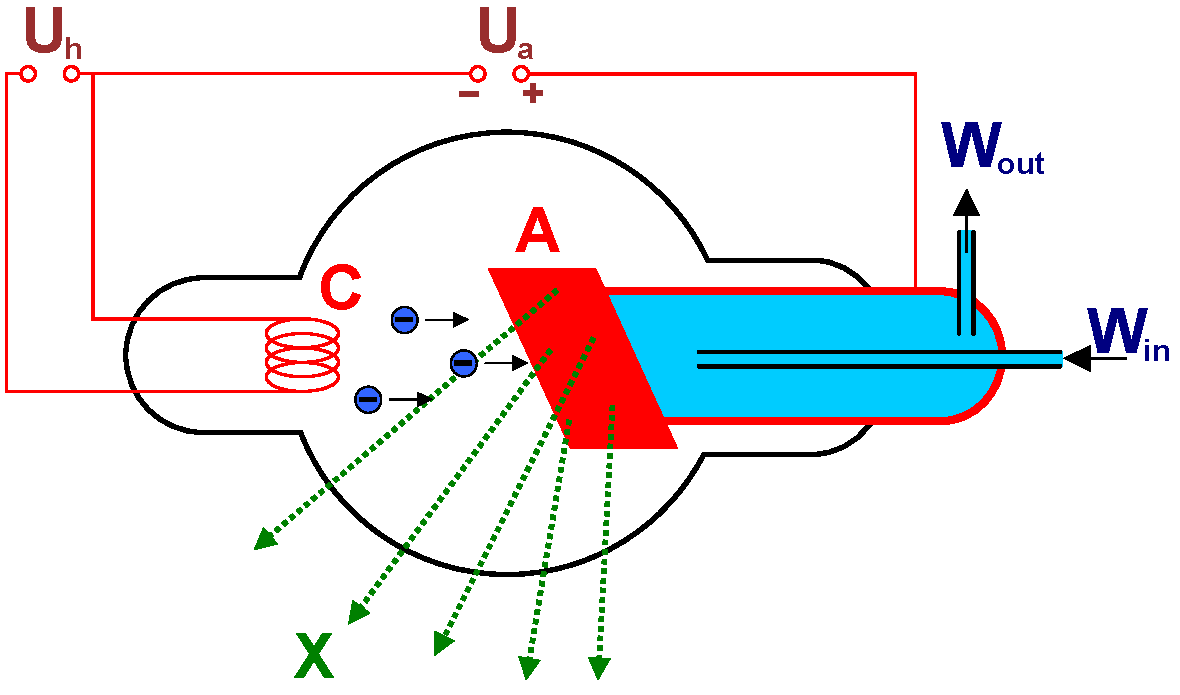
\includegraphics[width=0.5\textwidth]{Abbildungen/WaterCooledXrayTube.pdf}
%     \caption{}
%     \label{fig:Roentgenroehre}
% \end{figure}\\


\subsection{Kristallographie}
% \begin{table}[ht]
% 	\centering
% 	\caption{}
% 	\label{tab:Achsensysteme}
% 	\begin{tabular}{l l l l}
% 		\toprule
% 	 	\midrule
% 	\end{tabular}
% \end{table}\\

% *********************************************
% ***** KAPITEL 3 *****************************
% *********************************************
\section{Versuchsdurchführung} \label{sec:Versuchsdurchführung}

% *********************************************
% ***** KAPITEL 4 *****************************
% *********************************************
\newpage
\section{Ergebnisse und Diskussion}


% *********************************************
% ***** KAPITEL 4 *****************************
% *********************************************
\section{Zusammenfassung}


% ***** Literaturverzeichnis ******************

\begin{thebibliography}{xxx}
	\bibitem{Demtroeder}
	W. Demtröder: \textit{Experimentalphysik 3: Atome, Moleküle und Festkörper}. Springer Verlag Berlin Heidelberg 2009 (4. Auflage).
	\bibitem{Glocker}
	R. Glocker: \textit{Materialprüfung mit Röntgenstrahlen}. Springer Verlag Berlin Heidelberg New York 1985 (5. Auflage).
  \bibitem{Kleber}
	W. Kleber u.a.: \textit{Einführung in die Kristallographie}. Oldenbourg Wissenschaftsverlag 2010 (19. Auflage).
  \bibitem{Uschmann}
  I. Uschmann: \textit{FSU Fortgeschrittenenen Praktikum: Debye-Scherrer-Verfahren}, Fried\-rich-Schil\-ler-Uni\-versi\-tät Oktober 2013
  \bibitem{Roentgenroehre}
  Aufbau einer Röntgenröhre: \url{wikimedia.org/wiki/File:WaterCooledXrayTube.svg}. Stand: 20.10.2019
\end{thebibliography}

\end{document}
